\documentclass{beamer}
\usepackage{xcolor}
\usepackage[utf8]{inputenc}
\usepackage[english]{babel} 
\usepackage{listings}

\usepackage{parcolumns}


\usetheme{Madrid}
\usecolortheme{beaver}

\beamertemplatenavigationsymbolsempty

\renewcommand{\emph}{\textcolor{red}}

%------------------------------------------------------------
%This block of code defines the information to appear in the
%Title page
\title[Resource Sharing] %optional
{Enabling resource sharing in dataflow circuits}

\author[Marmet] % (optional)
{Axel Marmet}

\institute[EPFL] % (optional)

\date[2020] % (optional)

\begin{document}

%The next statement creates the title page.
\frame{\titlepage}


\begin{frame}
\frametitle{Table of Contents}
\tableofcontents
\end{frame}

\section{Introduction}
\begin{frame}{Dataflow Circuits}
    Dataflow circuits are ...
\end{frame}
\begin{frame}{Resource sharing}
    There are two problems when sharing resources
    \begin{enumerate}
        \item Finding where to share, hard because there is no predetermined schedule
        \item Share in a way that ensures correct and deadlock-free execution
    \end{enumerate}
\end{frame}
\section{Motivation}
\begin{frame}{Prerequisite information}
    We define occupancy as the amount of tokens a component holds in steady state divided by the maximum amount of tokens it can hold. We already know how to obtain this value.\footnotemark
    
      \footnotetext{Josipovic et al., Buffer placement and sizing for high-performance dataflow circuits, FPGA'20}
\end{frame}
\begin{frame}[fragile]
\frametitle{Motivation}
\begin{columns}[T]
    \begin{column}{0.45\textwidth}
 \newline
      \begin{itemize}
          \item New iteration every two clock cycles
          \item Each multiplier has an occupancy of $0.5$
          \item Using only one multiplier would not hurt performance but diminish size of circuit
      \end{itemize}
    \end{column}
    \begin{column}{0.1\textwidth}
    \end{column}
    \begin{column}{0.45\textwidth}
      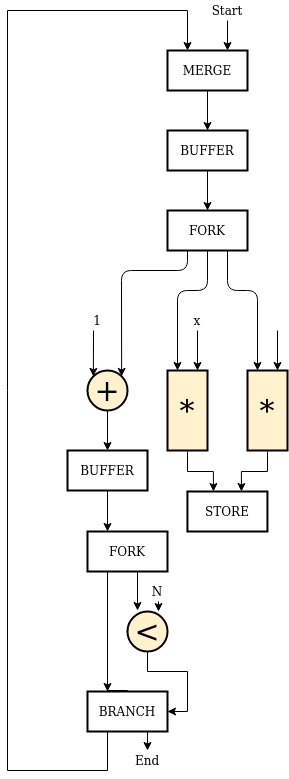
\includegraphics[scale=0.25]{base_case.png}
    \end{column}
  \end{columns}
\end{frame}

\begin{frame}[fragile]
\frametitle{Initial idea}
\begin{columns}[T]
    \begin{column}{0.45\textwidth}
    We add two new components to enable sharing \newline \newline
    \emph{Selector} \newline
    Responsible for selecting inputs in a way that ensures fairness and will never deadlock, augmented merge. 
    \newline 
    \newline
    \emph{Distributor} \newline
    Must send the resulting token to the correct outputs, is told where to send by the Selector  through a FIFO, augmented branch.
    \end{column}
    \begin{column}{0.1\textwidth}
    \end{column}
    \begin{column}{0.45\textwidth}
      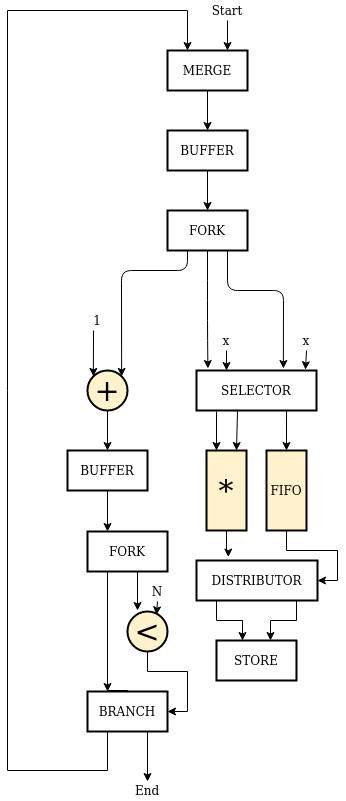
\includegraphics[scale=0.28]{shared_base_case.png}
    \end{column}
  \end{columns}
\end{frame}

\section{Deadlock avoidance}
\begin{frame}{Necessary transparent buffer in distributor}
    \begin{columns}[T]
    \begin{column}{0.45\textwidth}
    The distributor being able to hold the outputs is sometimes essential to allow the continuation of the computation. We enable this by using a 1 slot transparent buffer (TEHB)
    \end{column}
    \begin{column}{0.1\textwidth}
    \end{column}
    \begin{column}{0.45\textwidth}
      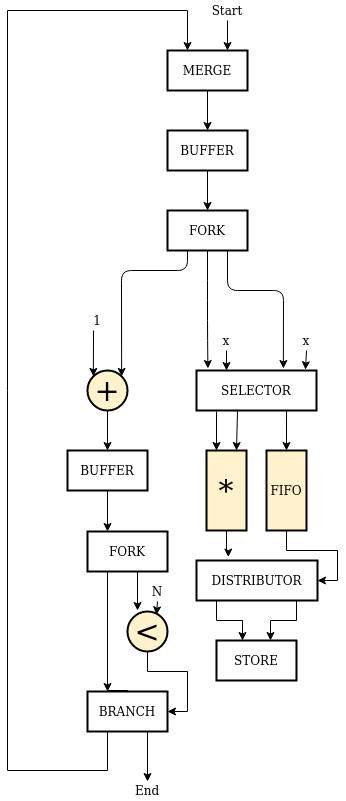
\includegraphics[scale=0.28]{shared_base_case.png}
    \end{column}
  \end{columns}
\end{frame}

%TODO add animation
\begin{frame}{Deadlock avoidance}
  How to schedule execution without causing deadlock ?
  \begin{columns}[T]
    \begin{column}{0.25\textwidth}
      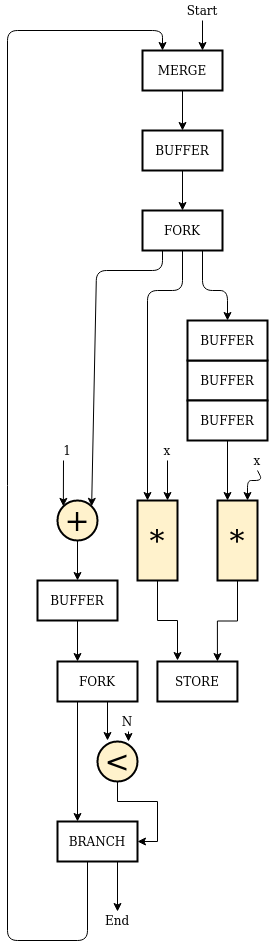
\includegraphics[scale=0.25]{blocking_unshared.png}
    \end{column}
    \begin{column}{0.1\textwidth}
    \begin{center}
        becomes
    \end{center}
    \end{column}
    \begin{column}{0.25\textwidth}
      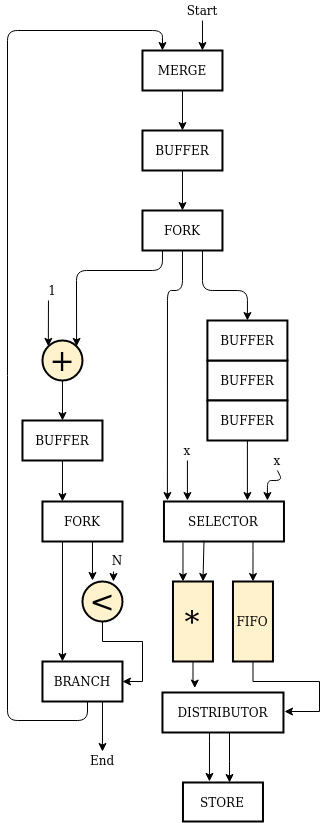
\includegraphics[scale=0.25]{blocking_shared.png}
    \end{column}
  \end{columns}
\end{frame}
\begin{frame}{Ordering}
\emph{Among BBs} \\
As the previous example highlighted we need to maintain an ordering among BBs. That is to say that all computations happening in one BB must be executed before any computations belonging to another BB begin. \newline \newline
\emph{Per BB} \\
We will also enforce an ordering among computations in the same BB. Although not strictly necessary it makes the sharing easier to model to the MILP.
\end{frame}

\begin{frame}{Modeling sharing to the MILP}
Two possibilities
\begin{enumerate}
    \item Modify shared components's latencies and initiation intervals
    \item Implement sharing using dataflow components
\end{enumerate}
\end{frame}

\begin{frame}{Enforcing all transactions firing}
\begin{columns}
    \begin{column}{0.45\textwidth}
    We must enforce that all transactions from one BB happen before any from another BB (or the same in another iteration) \newline \newline
    We use the same mechanism as LSQs to be informed of the order of execution of the BBs
    \end{column}
    \begin{column}{0.1\textwidth}
    \end{column}
    \begin{column}{0.45\textwidth}
      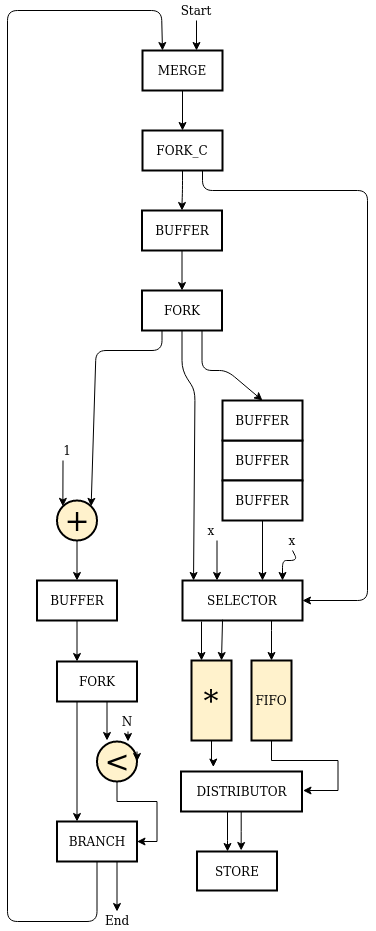
\includegraphics[scale=0.25]{blocking_shared_solution.png}
    \end{column}
  \end{columns}
\end{frame}

\begin{frame}{Ordering}
For optimal buffer placement we want to be able to somehow indicate to the MILP model that the components are shared. The first idea was to modify the latencies and initiation intervals. Not ideal because incrementing latency correctly is not trivial. The second idea is to add to the control path to explicitly enforce an order per BB. (There won't be a lengthy paragraph like that in the final presentation, this is just to show how I wanna structure it)
\end{frame}

\begin{frame}{Explicit ordering for MILP}
Nice picture here
\end{frame}

\section{Components}
\begin{frame}{Selector}
Todo
\end{frame}

\begin{frame}{Distributor}
    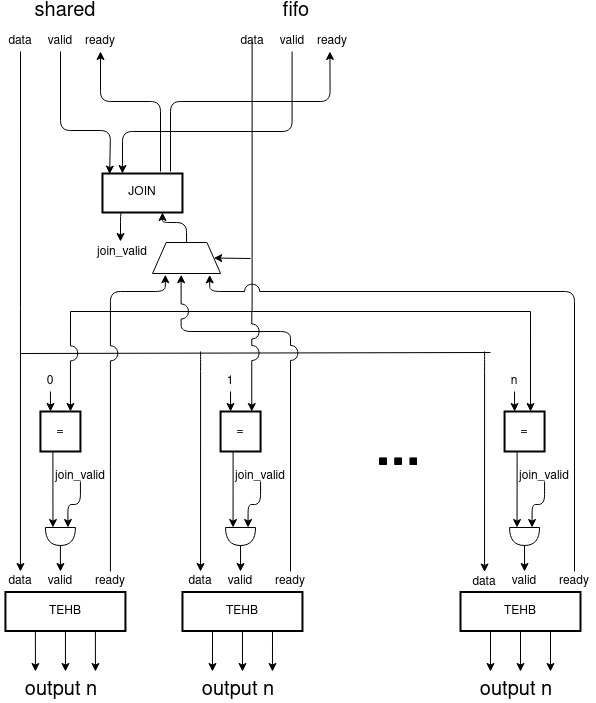
\includegraphics[scale=0.3]{distributor.png}
\end{frame}

\section{Algorithm}
\begin{frame}{Algorithm}
Simplified pseudocode algorithm
\end{frame}

\section{Next steps}
\begin{frame}{Next steps}
\begin{itemize}
    \item Find a heuristic or algorithm to find best ordering without exhaustive search
    \item Get quantitative results
\end{itemize}
\end{frame}

\end{document}